\documentclass[hyperref={pdfpagelayout=SinglePage}]{beamer}
\usetheme{Warsaw}
\usecolortheme{default}
\usefonttheme[onlymath]{serif}
\usepackage[utf8]{inputenc}
\usepackage[spanish,activeacute]{babel}

\usepackage{graphicx}
\usepackage{fancyhdr}
\usepackage{float}
\usepackage{adjustbox}
\usepackage{subfigure}
\usepackage{amsmath}
\usepackage{ragged2e}

\usepackage{color}
\usepackage{listings}
\lstset{ %
basicstyle=\tiny,       % the size of the fonts that are used for the code
numbers=none,                   % where to put the line-numbers
numberstyle=\footnotesize,      % the size of the fonts that are used for the line-numbers
stepnumber=1,                   % the step between two line-numbers. If it is 1 each line will be numbered
numbersep=5pt,                  % how far the line-numbers are from the code
backgroundcolor=\color{white},  % choose the background color. You must add \usepackage{color}
showspaces=false,               % show spaces adding particular underscores
showstringspaces=false,         % underline spaces within strings
showtabs=false,                 % show tabs within strings adding particular underscores
frame=single,           % adds a frame around the code
tabsize=4,          % sets default tabsize to N spaces
captionpos=b,           % sets the caption-position to bottom
breaklines=true,        % sets automatic line breaking
breakatwhitespace=false,    % sets if automatic breaks should only happen at whitespace
escapeinside={\%*}{*)}          % if you want to add a comment within your code
}
\renewcommand{\lstlistingname}{Código}
\renewcommand\spanishtablename{Tabla}

\expandafter\def\expandafter\insertshorttitle\expandafter{%
  \insertshorttitle\hfill%
  \insertframenumber\,/\,\inserttotalframenumber}

\usepackage{animate}

\title{Movimiento Browniano}
\subtitle{Trabajo Practico Nro. 3}
\author{Badi Leonel, Buchhalter Nicolás Demián y Meola Franco Román}
\subject{Simulación de Sistemas}
\date{\today}

\makeatletter
\@addtoreset{subfigure}{framenumber}
\makeatother

\begin{document}

\renewcommand{\figurename}{Grafico}

\begin{frame}[plain]
    \frametitle{} 
    \titlepage
    \centering
	Grupo 3
\end{frame}

\section{Fundamentos}

\subsection{Introducción}

\begin{frame}
\frametitle{Fundamentos}
\framesubtitle{Introducción}
\begin{itemize}
	\item Movimiento Browniano
	\item Dinámica molecular dirigida por eventos con choques elásticos
	\item Las partículas siguen un movimiento rectilíneo uniforme entre colisiones
\end{itemize}
\end{frame}

\subsection{Variables relevantes}

\begin{frame}
\frametitle{Fundamentos}
\framesubtitle{Variables relevantes}
\begin{itemize}
	\item $N$ : número de partículas
	\item Dominio cuadrado de $0.5 m$ de lado
	\item \textbf{$N$ partículas pequeñas}
	\begin{itemize}
		\item $R_{1} = 0.005 m$
		\item $m_{1} = 1 kg$
	\end{itemize}
	\item \textbf{Una partícula grande}
	\begin{itemize}
		\item $R_{2} = 0.05 m$
		\item $m_{2} = 100 kg$
	\end{itemize}
\end{itemize}
\end{frame}

\section{Implementación}

\subsection{Generación de los agentes}

\begin{frame}
\frametitle{Implementación}
\framesubtitle{Generación de los agentes}
\begin{itemize}
	\item Posiciones $(x,y)$ aleatorias para todas las partículas evitando la superposición de las mismas
	\item $-0.1 \frac{m}{s} < v_{0} < 0.1 \frac{m}{s}$ en $x$ e $y$ para las partículas chicas
	\item $v_{0} = 0$ para la partícula grande
	\item Todas las paredes son rígidas
\end{itemize}
\end{frame}

\subsection{Simulación}

\begin{frame}
\frametitle{Simulación}
\framesubtitle{Variables relevantes}
\begin{itemize}
	\item $dt$ intrínseco variable
	\item $dt2$ constante
	\item \texttt{time} : Tiempo en segundos a visualizar
	\item $dt2 =$ \texttt{frameRate} : Número de frames por segundo
\end{itemize}
\end{frame}

\begin{frame}[fragile]
\frametitle{Implementación}
%\framesubtitle{Simulación}
\begin{lstlisting}[language=Java, caption = Función para obtener el tiempo de la próxima colisión.]
public double timeToNextColision(){
	Double t = Double.MAX_VALUE;
	for(int i = 0; i < N; j++){
		Particle particle = getParticle(i);
		Double calculatedTime = timeToBorder(particle, t);
		if(calculatedTime < t){
			t = calculatedTime;
		}
		for(int j = i+1 ; j < N; j++){
			Particle particle2 = getParticle(j);
			if(!particle.equals(particle2)) {
				if (calculateD(particle,particle2) >= 0) {
					if (calculatedTime(particle,particle2) < t) {
						colParticle1 = particle;
						colParticle2 = particle2;
						t = calculatedTime;
					}
				}
			}
		}
	}
	return t;
}
\end{lstlisting}
\end{frame}


\begin{frame}[fragile]
\frametitle{Implementación}
%\framesubtitle{Simulación}
\begin{lstlisting}[language=Java, caption = Algoritmo de simulación del sistema.]
public void simulate(double time, double frameRate){
	writeFrame();
	while(time > 0){
		accumulatedTime += timeToNextCollision();
		if(accumulatedTime < frameRate) {
			moveSystem(timeToNextCollision);
			collide(particle1, particle2); //particle2 == null cuando es borde
		} else {
			moveSystem(frameRate - (accumulatedTime - timeToNextCollision));
			writeFrame();
			time -= frameRate;
			for(j=2*frameRate; j<accumulatedTime && time> 0; j+=frameRate) {
				time -= frameRate;
				moveSystem(frameRate);
				writeFrame();
			}
			moveSystem(accumulatedTime - (j - frameRate));
			accumulatedTime = 0;
		}
	}
}
\end{lstlisting}
\end{frame}

\begin{frame}
\frametitle{Implementación}
\framesubtitle{Problemas encontrados}
\begin{itemize}
\item Precisión del \texttt{double}: Al colisionar con bordes obtuvimos \texttt{timeToNextCollision} negativos
\item Utilización de una heurística: Cell Index Method resultó muy costoso, aumentando el tiempo necesario para la simulación con los valores de $N$ probados.
\end{itemize}
\end{frame}

\subsection{Visualización}

\begin{frame}
\frametitle{Implementación}
\framesubtitle{Visualización}
\begin{itemize}
	\item La simulación y la visualización son independientes
	\item El algoritmo de simulación escribe un archivo \texttt{.tsv} con los siguientes datos:
\begin{itemize}
\item $(x,y)$
\item $r$
\item Color RGB para indicar las velocidades, donde R es la componente en el eje Y y G es la componente en eje X
\end{itemize}
\item Por último, se carga en \texttt{Ovito} el archivo de salida\texttt{.tsv} para realizar la visualización
\end{itemize}
\end{frame}

\section{Resultados}

\subsection{Tablas y Gráficos}

\begin{frame}
\frametitle{Resultados}
\framesubtitle{Tiempo promedio para el cálculo de la simulación para distintos valores de $N$}
\begin{center}
\begin{table}[h]
\centering
\adjustbox{max height=\dimexpr\textheight-3.0cm\relax,
           max width=\textwidth}{
\begin{tabular}{cc}
\hline
\textbf{$N$} & \textbf{$t$}\\ \hline
10&342 ms\\
100&4 seg\\
250&1 min 12 seg\\
500&18 min\\
1000&6hs 12 min\\
\end{tabular}
}
\caption{Tiempo promedio para el cálculo de la simulación para distintos valores de $N$.}
\end{table}
\end{center}
\end{frame}

\begin{frame}
\frametitle{Resultados}
\framesubtitle{Gráfico Frecuencia de colisiones}
\begin{figure}[H]
        \centering
        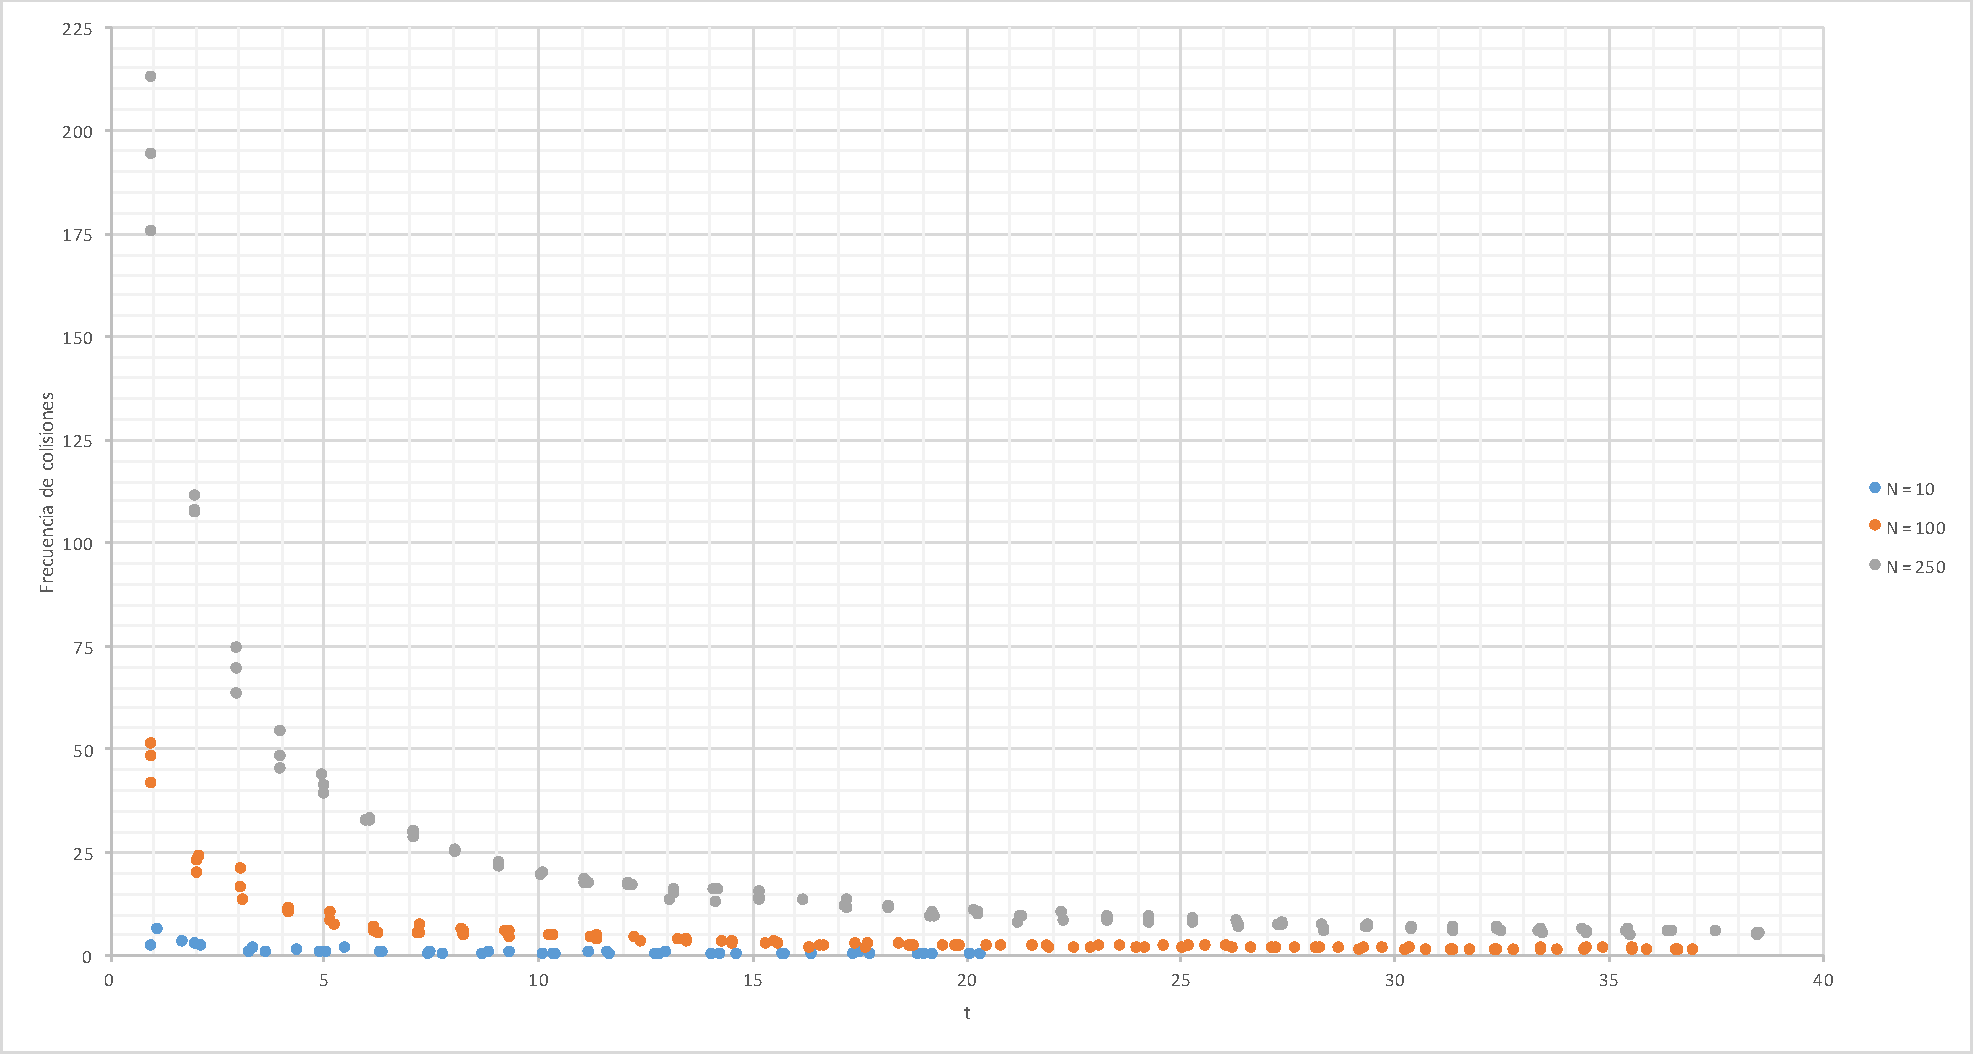
\includegraphics[width=\textwidth]{Frecuenciaxt.pdf}
        \caption{Gráfico de la frecuencia de colisiones por unidad de tiempo}
\end{figure}
\end{frame}

\begin{frame}
\frametitle{Resultados}
\framesubtitle{Frecuencia de colisiones para distintos valores de $N$}
\begin{center}
\begin{table}[h]
\centering
\adjustbox{max height=\dimexpr\textheight-3.0cm\relax,
           max width=\textwidth}{
\begin{tabular}{cc}
\hline
\textbf{$N$} & \textbf{$f \frac{colisiones}{s}$}\\ \hline
10&0,76\\
100&5,25\\
250&22,33\\
500&86,3\\
1000&466,75\\
\end{tabular}
}
\caption{Frecuencia de colisiones para distintos valores de $N$.}
\end{table}
\end{center}
\end{frame}

\begin{frame}
\frametitle{Resultados}
\framesubtitle{Gráfico de la distribución de velocidades}
\begin{figure}[H]
        \centering
        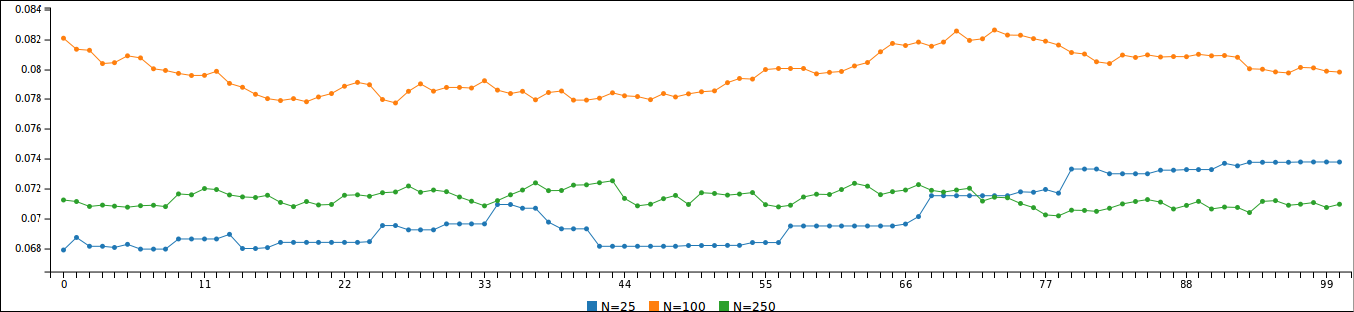
\includegraphics[width=\textwidth]{graphs/velocities.png}
        \caption{Gráfico de la distribución de velocidades en el último tercio de la simulación}
\end{figure}
\end{frame}

\begin{frame}
\frametitle{Resultados}
\framesubtitle{Gráfico de la trayectoria de la partícula grande}
  \hfil\hfil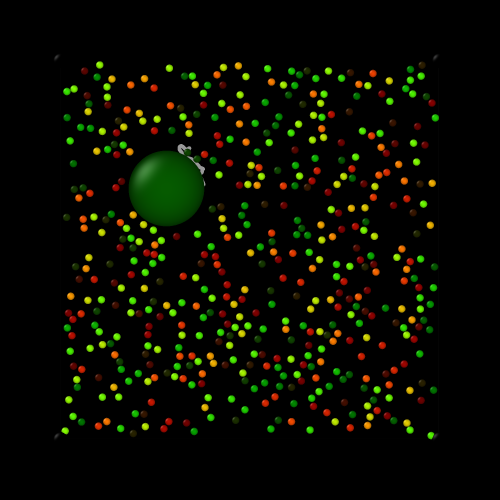
\includegraphics[width=5cm]{500v1.png}\hfil\hfil
    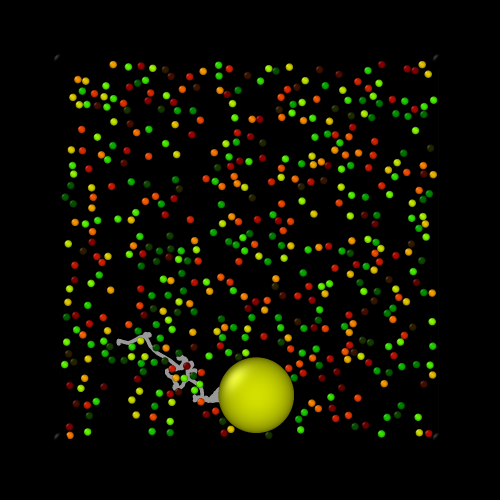
\includegraphics[width=5cm]{500v2.png}\newline
  \null\hfil\hfil\makebox[5cm]{$|v_{0}| = 0.1 \frac{m}{s}$}
    \hfil\hfil\makebox[5cm]{$|v_{0}| = 0.5 \frac{m}{s}$}
\end{frame}

\begin{frame}
\frametitle{Resultados}
\framesubtitle{Gráfico de la trayectoria de la partícula grande}
\begin{figure}[H]
        \centering
        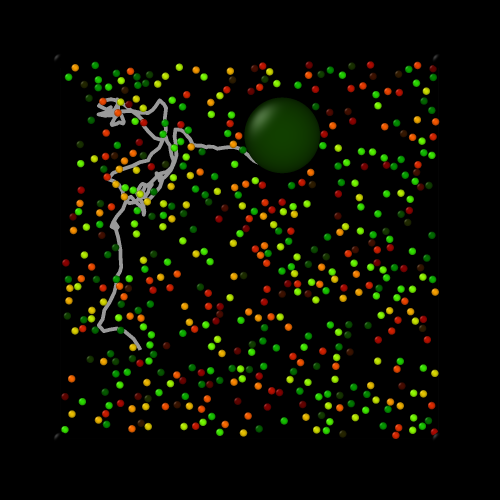
\includegraphics[width=5cm]{500v3.png}
        \caption{Trayectoria de la partícula grande con $|v_{0}| = 1 \frac{m}{s}$}
\end{figure}
\end{frame}

\subsection{Animaciones}

\begin{frame}
\frametitle{Resultados}
\framesubtitle{Animación de la simulación para $N = 100$}
\begin{figure}[H]
	\centering
	\animategraphics[loop,controls,width=0.75\textheight]{10}{animation/dmer-100-}{0000}{0200}
\end{figure}
\end{frame}

\begin{frame}
\frametitle{Resultados}
\framesubtitle{Animación de la simulación para $N = 500$}
\begin{figure}[H]
	\centering
	\animategraphics[loop,controls,width=0.75\textheight]{10}{animation/dmer-500-}{0000}{0200}
\end{figure}
\end{frame}

\begin{frame}
\frametitle{Resultados}
\framesubtitle{Animación de la simulación para $N = 1000$}
\begin{figure}[H]
	\centering
	\animategraphics[loop,controls,width=0.75\textheight]{10}{animation/dmer1000-}{0000}{0200}
\end{figure}
\end{frame}

\subsection{Conclusiones}

\begin{frame}
\frametitle{Conclusiones}
\begin{itemize}
	\item Aumentando la energía cinética se puede simular un aumento en la temperatura. $K = n R T$
	\item Con $N = 1000$ el comportamiento se asemeja a un material viscoso, existiendo un límite definido por las dimensiones del dominio.
	\item A mayor $N$ la partícula grande se desplaza menos.
	\item Aumentando la velocidad de las partículas, aumentan la frecuencia de colisión y el tiempo de procesamiento.
	\item El sistema no se estabiliza ya que todas las fuerzas son conservativas.
\end{itemize}
\end{frame}

\begin{frame}[plain,c]
\begin{center}
	\Huge Gracias
\end{center}
\end{frame}

\end{document}